\subsubsection{Objectives and Requirements}
The goal of our global planner is to compute, at runtime, a collision-free route from the robot’s current pose to the next tower in the Tower Dropper scenario. The planner must respect:
\begin{itemize}
  \item \textbf{Static environment:} a 5\,m × 5\,m occupancy grid (5\,cm resolution) generated by our mock map publisher.
  \item \textbf{Robot footprint:} approximated as a circle of radius 0.3\,m, enforced via obstacle inflation.
  \item \textbf{Real-time constraints:} paths should be available within a few hundred milliseconds to allow seamless integration with our local controller and to react promptly when the mock publisher advances to the next tower.
\end{itemize}

\subsubsection{Algorithm Selection and Design}
We surveyed classic grid-based planners (Dijkstra for guaranteed optimality, RRT for sampling-based routes) but settled on \textbf{A*} on an occupancy grid for its simplicity and determinism. In our \texttt{PathPlannerNode}:
\begin{enumerate}
  \item \textbf{Grid representation:} a 2D \texttt{NumPy} array of occupancy values (0 = free, $\geq$50 = occupied).
  \item \textbf{Search:} an 8-connected A* using a min-heap (\texttt{heapq}) keyed by $f = g + h$, where $g$ is accumulated path cost and $h$ the Euclidean distance to goal. Orthogonal moves cost 1; diagonal moves cost $\sqrt{2}$. Corner-cutting checks prevent invalid diagonals.
  \item \textbf{Path pruning:} after finding the raw A* path, we remove unnecessary waypoints by testing straight-line visibility with a Bresenham-based \texttt{\_has\_los} check.
\end{enumerate}

\subsubsection{Map Representation, Visualization \& Preprocessing}
To debug and tune our planner, we relied heavily on \texttt{RViz2}, subscribing to the \texttt{/map} and \texttt{/plan} topics to inspect both the occupancy grid and computed paths in real time. Figures~\ref{fig:raw-pruned} and~\ref{fig:inflated} illustrate this process.

\begin{figure}[ht]
  \centering
  \begin{minipage}[b]{0.24\textwidth}
    \centering
    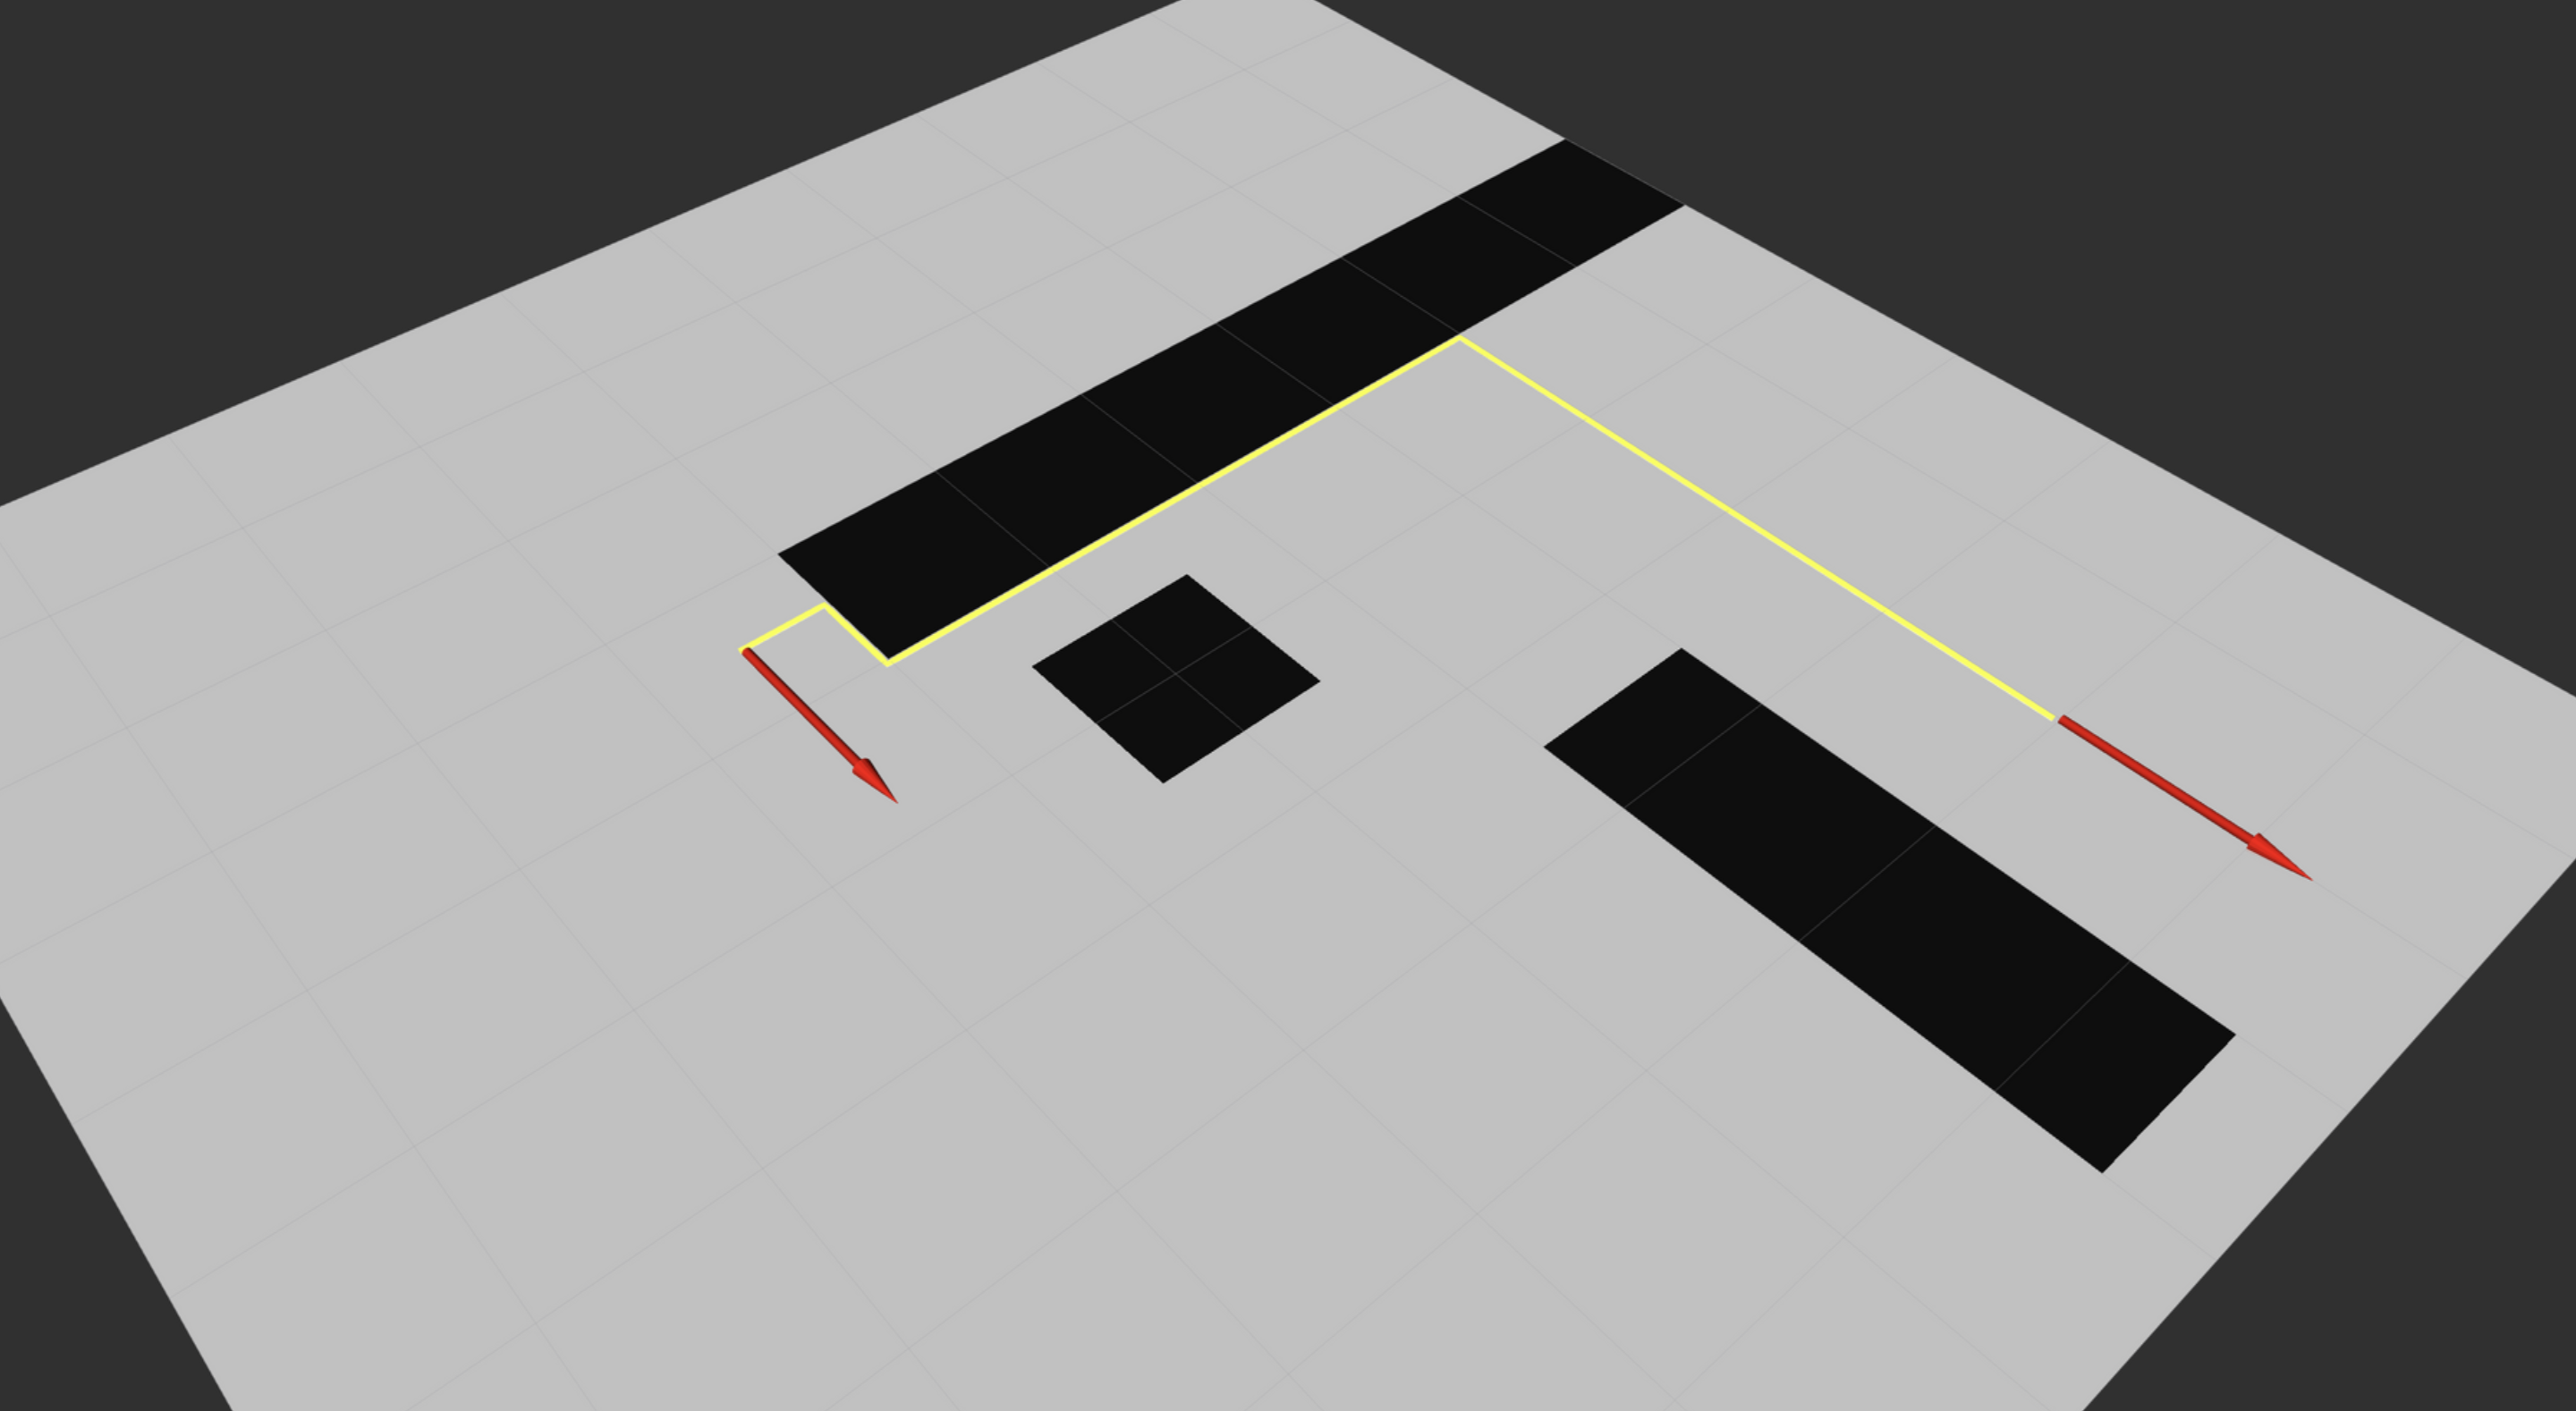
\includegraphics[width=\linewidth]{Images/path1.png}
  \end{minipage}
  \hfill
  \begin{minipage}[b]{0.24\textwidth}
    \centering
    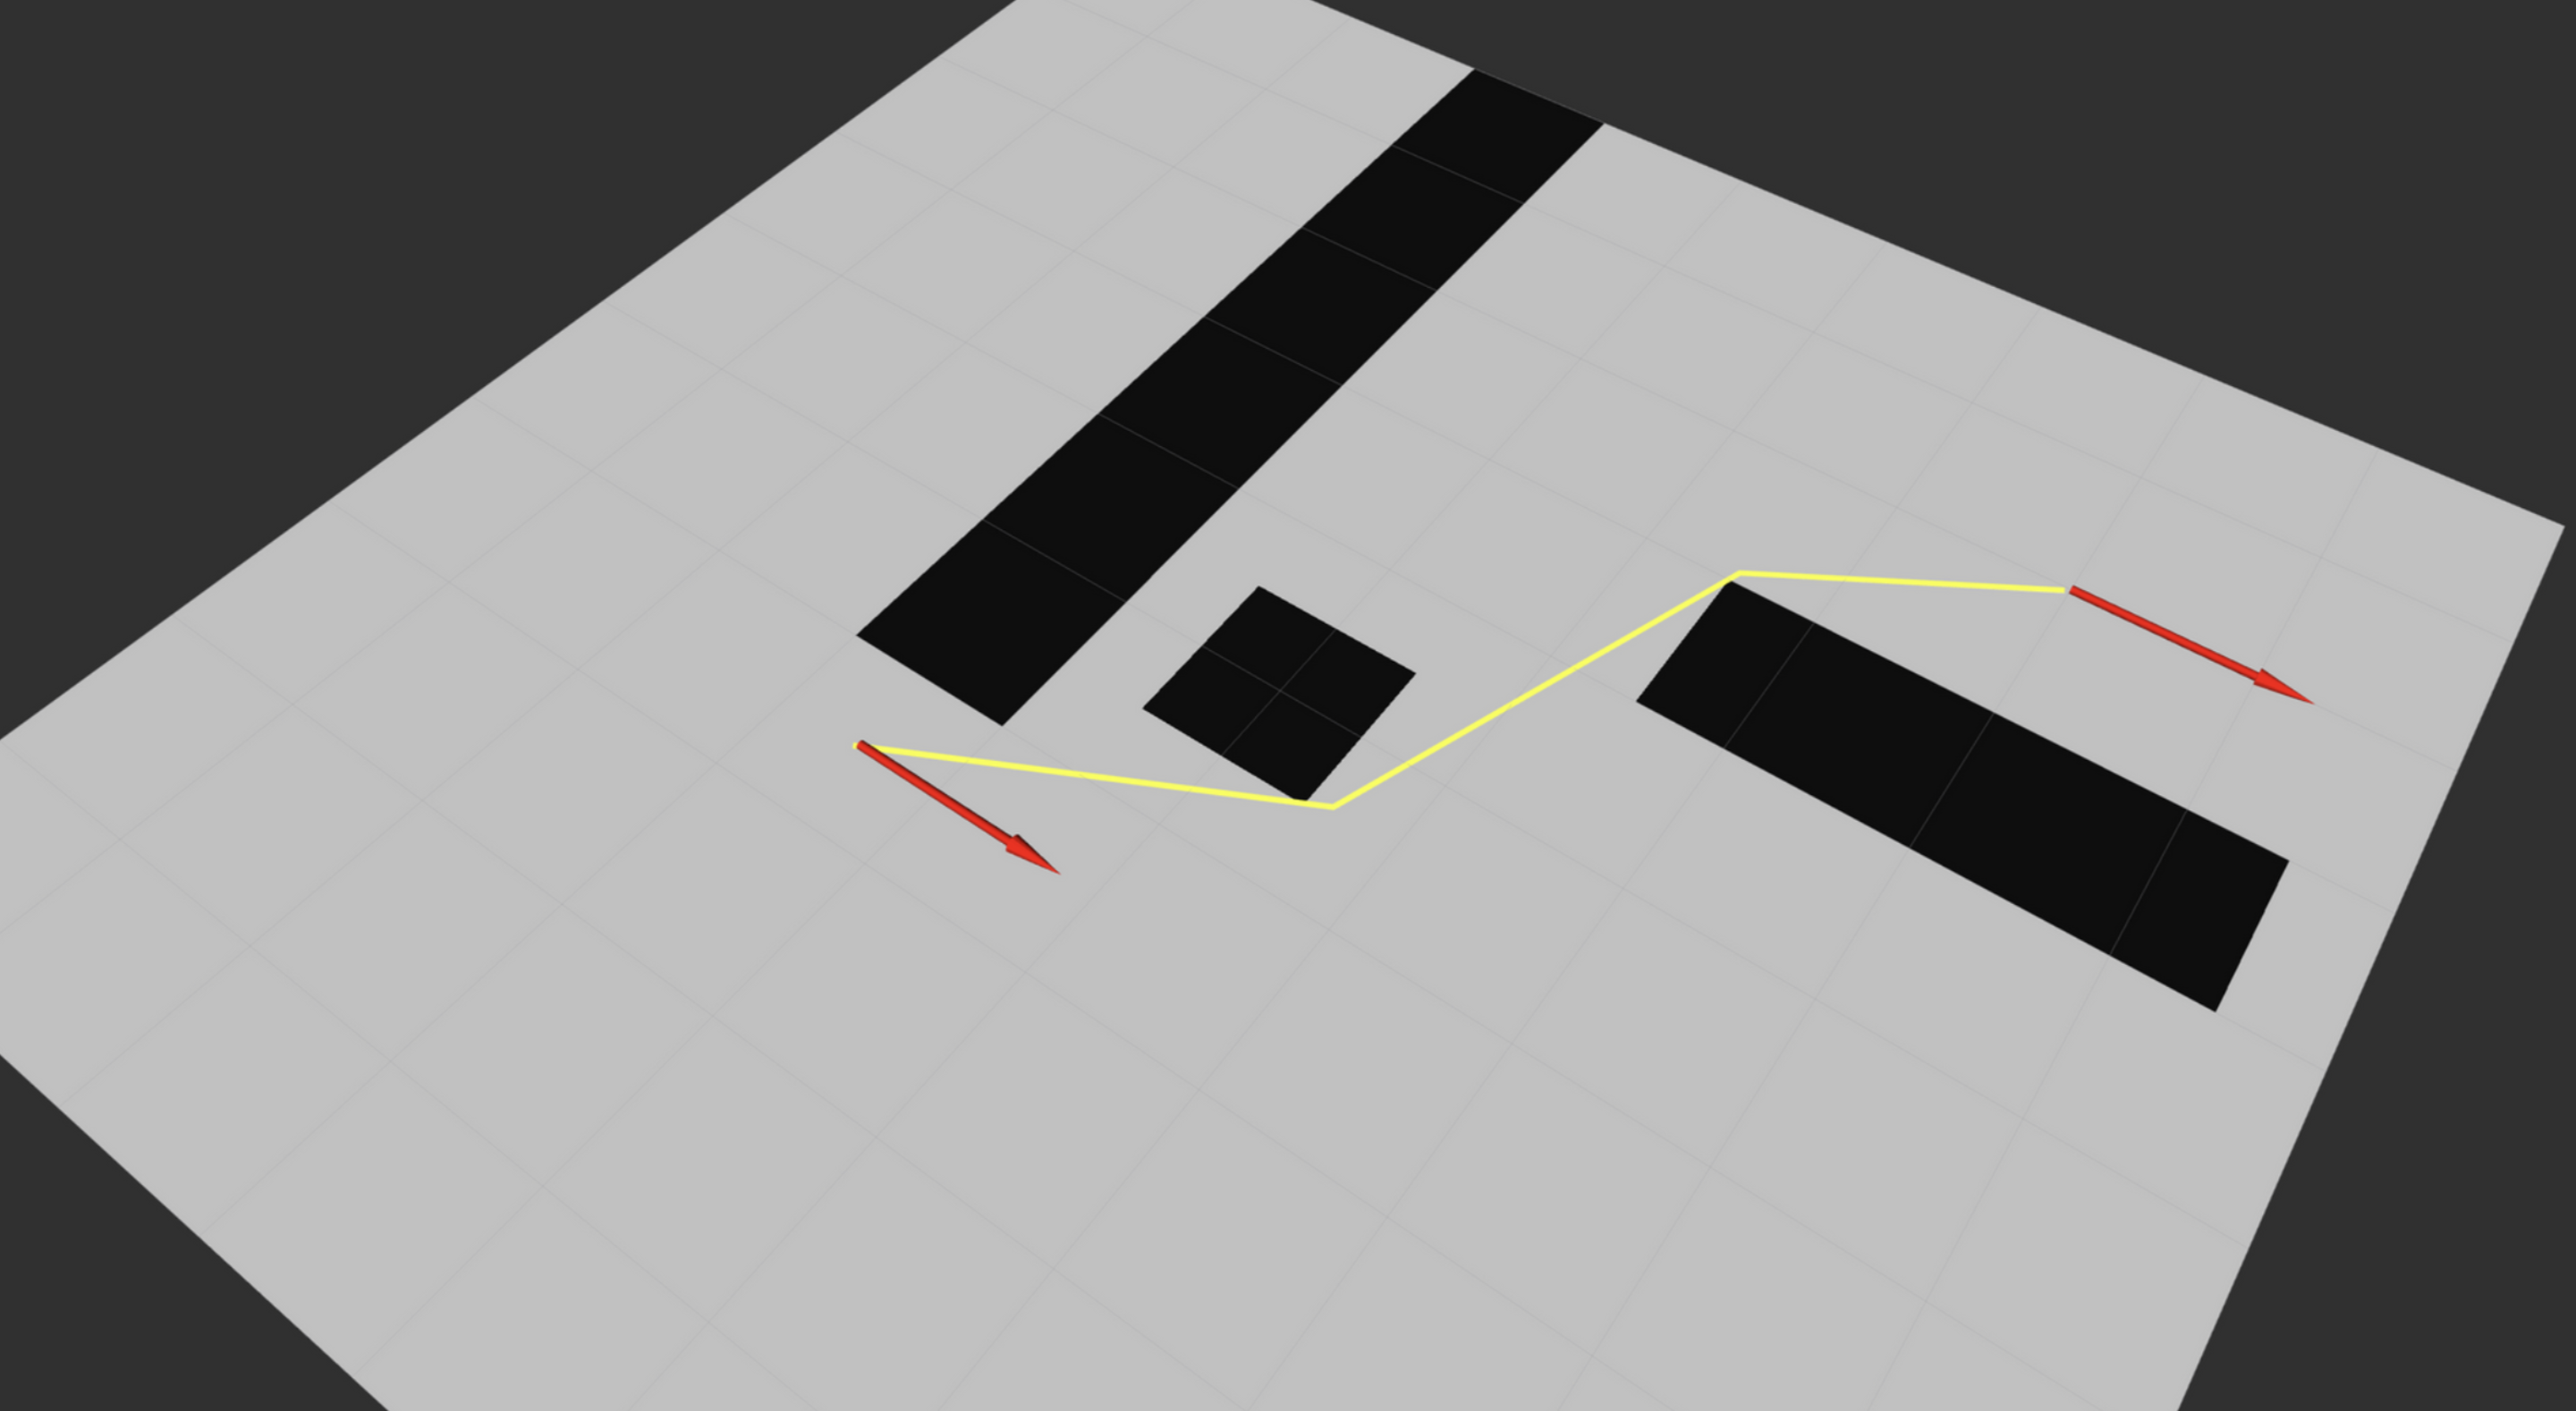
\includegraphics[width=\linewidth]{Images/path2.png}
  \end{minipage}
  \caption{Initial pathfinding: left—raw A* solution; right—after line-of-sight pruning.}
  \label{fig:raw-pruned}
\end{figure}

Subsequently, we introduced obstacle inflation to enforce the robot’s safety margin and avoid corner collisions:

\begin{figure}[ht]
  \centering
  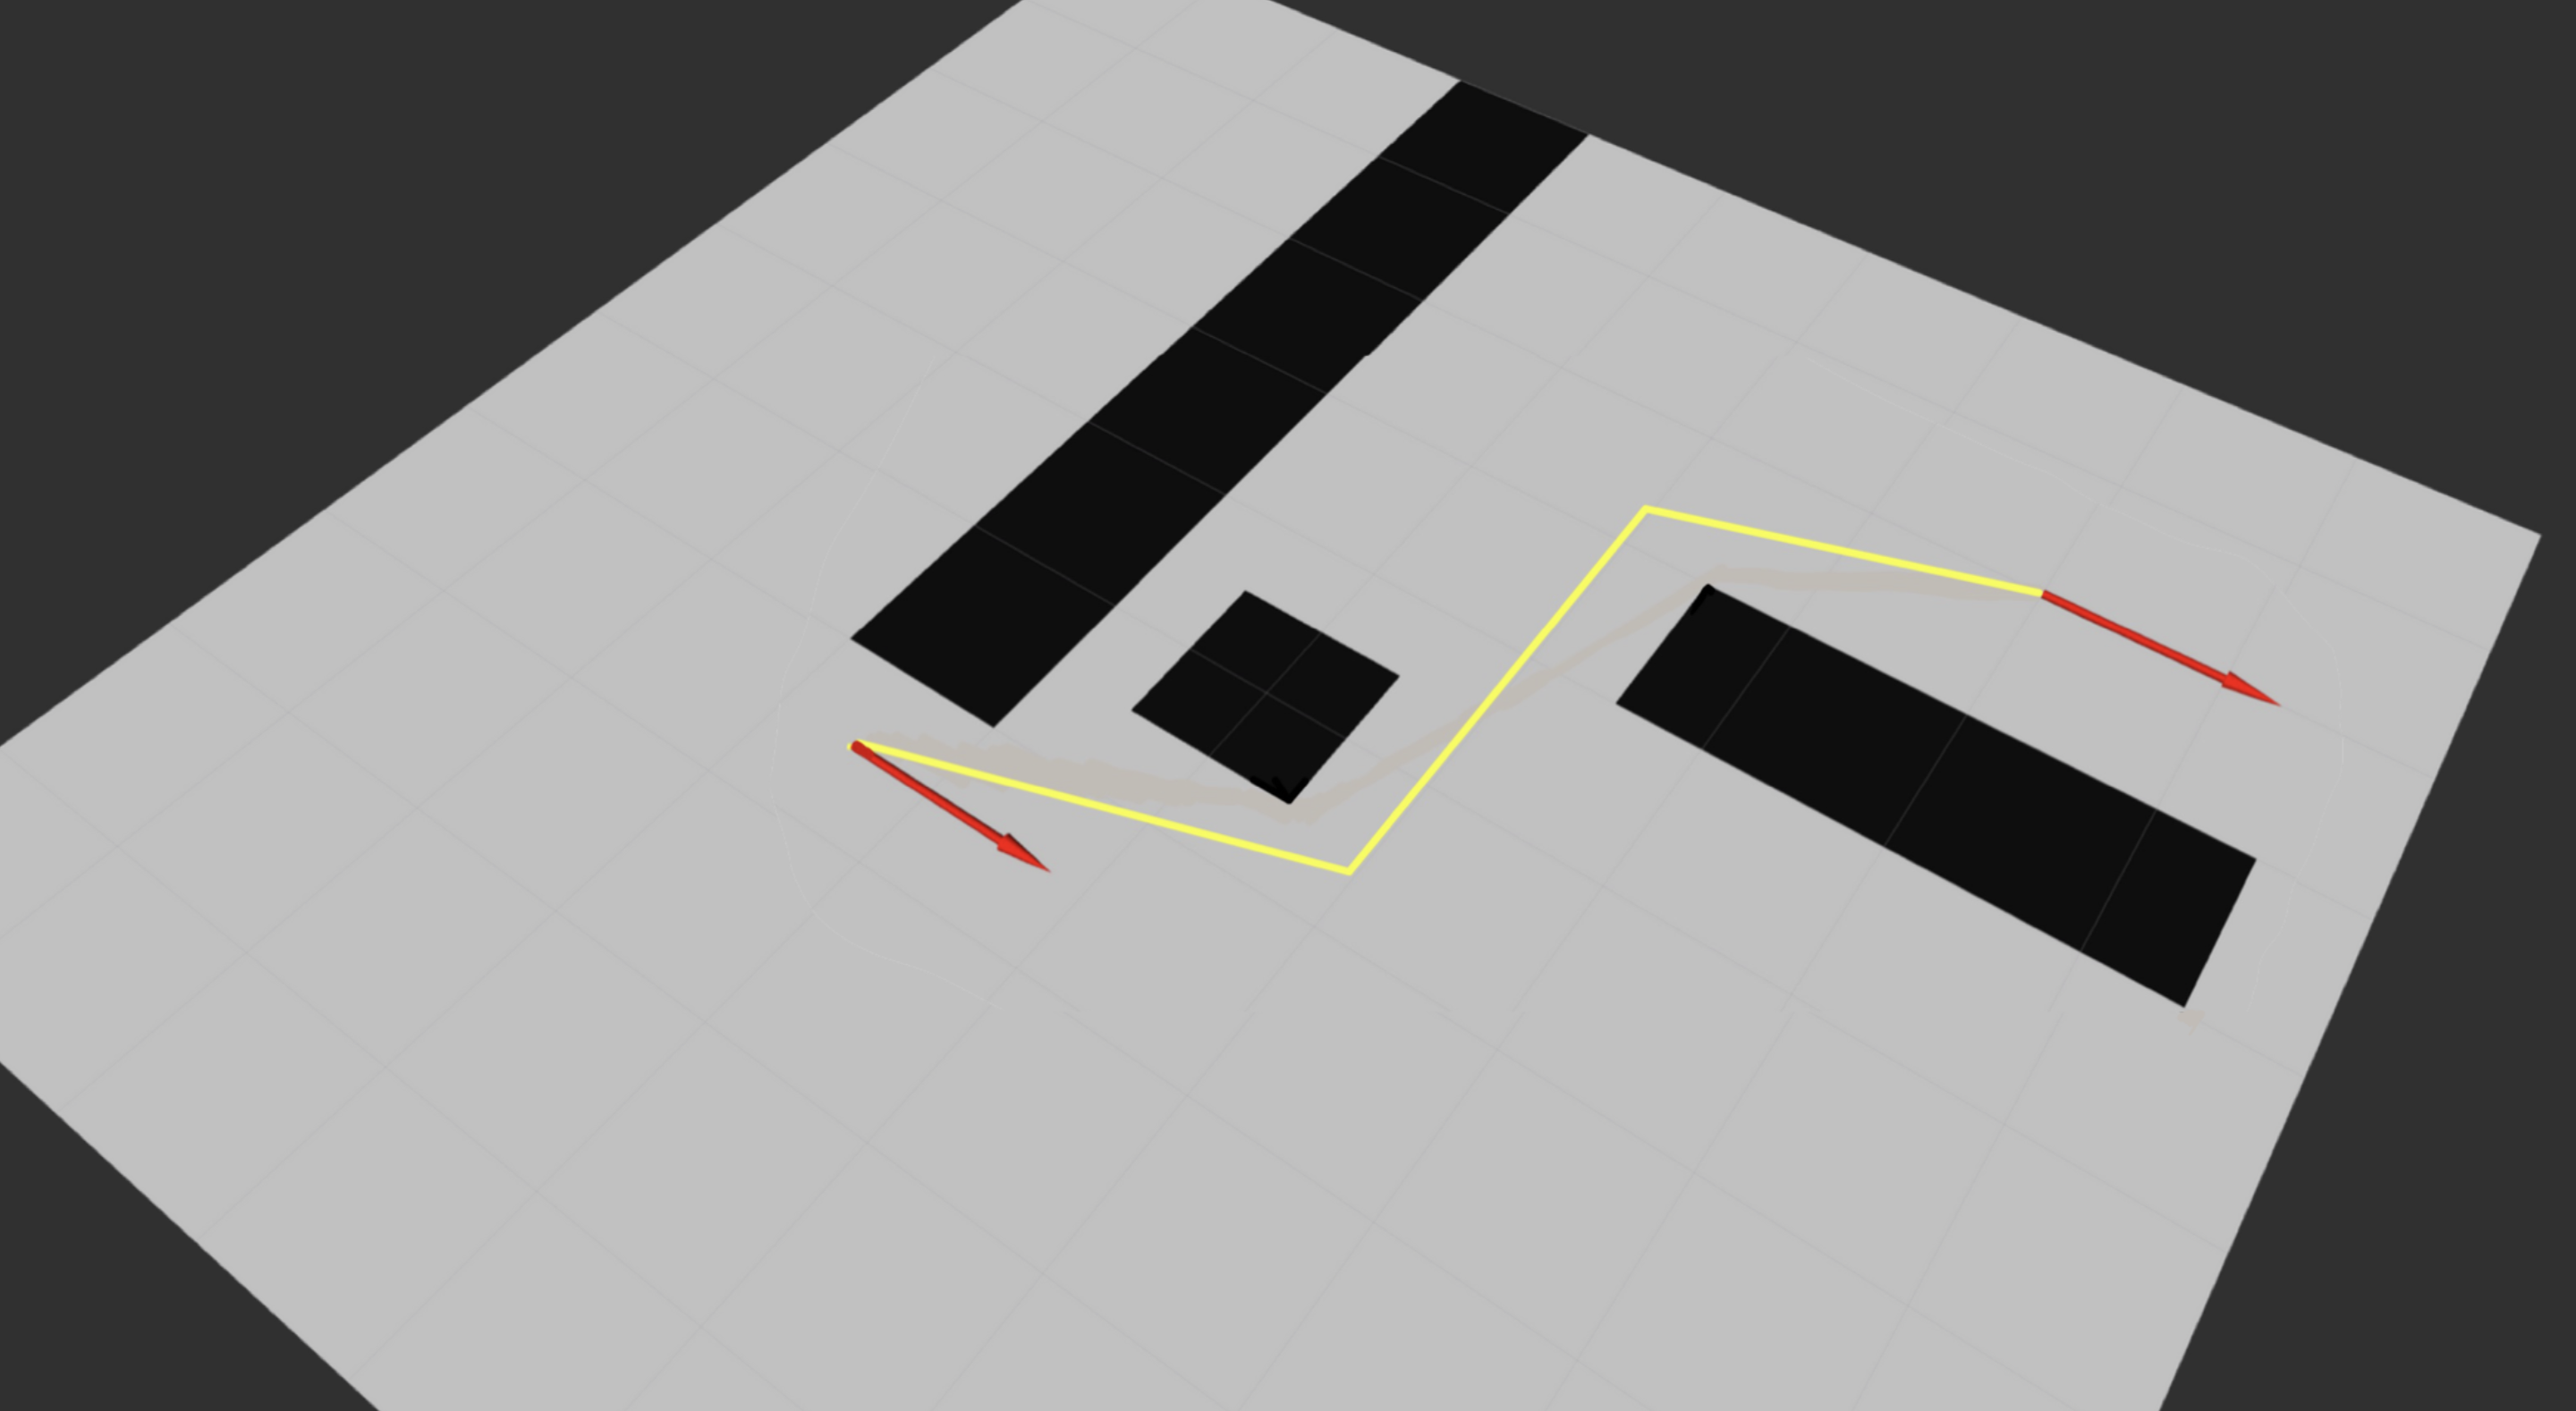
\includegraphics[width=0.4\textwidth]{Images/path3.png}
  \caption{Pathfinding on the inflated map (beige overlay): the planner keeps clear of obstacle edges.}
  \label{fig:inflated}
\end{figure}

\noindent\textbf{Preprocessing steps:}
\begin{itemize}
  \item Reshape \texttt{OccupancyGrid.data} into a 2D array.
  \item Inflate each occupied cell by 
    \texttt{inflate\_radius = int(0.3 / resolution)} 
    to mark neighboring cells as occupied, ensuring collision clearance.
\end{itemize}

\subsubsection{ROS2 Integration}
The planner is implemented as a ROS 2 node with:
\begin{description}
  \item[Subscriptions:] 
    \texttt{/map} (\texttt{OccupancyGrid}), 
    \texttt{/goal\_pose} (\texttt{PoseStamped}), 
    \texttt{/rm0/odom} (\texttt{Odometry}), 
    \texttt{/go\_again}, \texttt{/goal\_reached} (\texttt{Bool}).
  \item[Publishers:] 
    \texttt{/plan} (\texttt{nav\_msgs/Path}), 
    \texttt{/current\_pose} (\texttt{PoseStamped}), 
    \texttt{/rm0/cmd\_vel} (\texttt{Twist}), 
    \texttt{/goal\_reached} (\texttt{Bool}).
  \item[TF Broadcast:] emits an \texttt{odom → base\_link} transform each update, plus a \texttt{static\_transform\_publisher} for \texttt{map → odom} to align frames in RViz.
  \item[Namespace handling:] launch with \texttt{--namespace <robot>} so one codebase runs on multiple robots unchanged.
\end{description}

\subsubsection{Issues Encountered \& Troubleshooting}
\begin{description}
  \item[TF frame misalignment] 
    \textit{Symptom:} paths appeared shifted in RViz.  
    \textit{Diagnosis:} no \texttt{map → odom} static transform in \texttt{/tf}.  
    \textit{Solution:} added a \texttt{static\_transform\_publisher} in the launch file to broadcast an identity \texttt{map → odom}.
  \item[Unknown-cell “blockades”] 
    \textit{Symptom:} planner routed through unexplored (–1) cells on SLAM maps.  
    \textit{Diagnosis:} we treated –1 as free in our occupancy threshold.  
    \textit{Solution:} in \texttt{map\_cb}, mark any \texttt{grid[y][x] < 0} as 100 before inflation, treating unknown as occupied.
  \item[Occupied goal cell handling] 
    \textit{Symptom:} when running the tower-knockdown process, the robot sometimes started inside a region forbidden by the inflated map, causing “no path found.”  
    \textit{Diagnosis:} both start and goal cells were disallowed by inflation.  
    \textit{Solution:} implemented \texttt{\_nearest\_free(goal\_cell)}, which performs an orthogonal BFS to locate the closest free cell; we then replace the goal with that cell and replan automatically.
\end{description}
